%!TEX TS-program = xelatex
\documentclass[]{friggeri-cv}
\usepackage{afterpage}
\usepackage{hyperref}
\usepackage{color}
\usepackage{xcolor}
\usepackage[most]{tcolorbox}
\usepackage[table]{xcolor}
\usepackage{tikz}
\usepackage{blindtext}
\usepackage{soul}
\usepackage[contents={},opacity=0]{background}

\DeclareRobustCommand{\hlcyan}[1]{{\sethlcolor{cyan}\hl{#1}}}


\hypersetup{
    pdftitle={},
    pdfauthor={},
    pdfsubject={},
    pdfkeywords={},
    colorlinks=false,       % no lik border color
   allbordercolors=white    % white border color for all
}
\tcbset{
    frame code={}
    center title,
    left=0pt,
    right=0pt,
    top=0pt,
    bottom=0pt,
    colback=gray!70,
    colframe=white,
    width=\dimexpr\textwidth\relax,
    enlarge left by=0mm,
    boxsep=10pt,
    arc=0pt,outer arc=0pt,
    }



\RequirePackage{xcolor}
\definecolor{pblue}{HTML}{000000}%{0395DE}% %

\begin{document}

\header{Elias}{ Sepuru}
      {\centering{ Electrical \& Information Engineering Honours Student}}
      
% Fake text to add separator      
\fcolorbox{white}{gray}{\parbox{\dimexpr\textwidth-2\fboxsep-2\fboxrule}{%
.....
}}

% In the aside, each new line forces a line break
\begin{aside}

%\begin{tcolorbox}

 \vspace{2.2cm}
  \section{Address}
  
   Block 21 Junction Ave,
   Parktown,
   Johannesburg,
   2193
    ~
  \section{Contact Details}
    Cell: 076 602 5334
    Home: 011 717 0498
    \href{mailto:eliassepuru@gmail.com}{{eliassepuru@gmail.com}}
    ~
  %\section{Mail}
  %  \href{mailto:eliassepuru@gmail.com}{{eliassepuru@gmail.com}}
  %  ~
  \section{Git \& LinkedIn}
  
\includegraphics[scale=0.025]{img/git.png}  \href{https://github.com/sephoro}{github.com/sephoro}
  \vspace{0.5cm} 
  
\includegraphics[scale=0.023]{img/linked2.png}
    \href{https://www.linkedin.com/in/elias-sepuru-30b931153/}{linkedin.com/in/elias-sepuru-30b931153}
    ~
  %\section{Programming}
  %  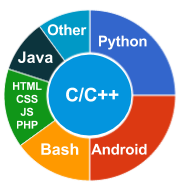
\includegraphics[scale=0.62]{img/programming.png}
  
    \section{Languages}
    \textbf{English}\hspace{0.5mm}$\>\>\>$
\includegraphics[scale=0.40]{img/5stars.png}
    \textbf{Sepedi}$\>\>\>\>\>$
\includegraphics[scale=0.40]{img/5stars.png}
    ~
 \section{Programming}
    \textbf{C++}\hspace{0.9cm}
\includegraphics[scale=0.4]{img/5stars.png}
    \textbf{C} \hspace{1.23cm}
\includegraphics[scale=0.40]{img/5stars.png}
    \textbf{JS}\hspace{1.14cm}
\includegraphics[scale=0.40]{img/5stars.png}
    \textbf{HTML}\hspace{0.60cm}
\includegraphics[scale=0.40]{img/5stars.png}
    \textbf{MATLAB}\hspace{0.12cm}
\includegraphics[scale=0.40]{img/5stars.png}
    \textbf{\LaTeX}\hspace{0.78cm}
\includegraphics[scale=0.40]{img/4stars.png}
    \textbf{Python}\hspace{0.39cm}
\includegraphics[scale=0.40]{img/3stars.png}
    \textbf{SQL}\hspace{0.88cm}
\includegraphics[scale=0.40]{img/3stars.png}
    \textbf{Assembly}\hspace{-0.02cm}
\includegraphics[scale=0.40]{img/3stars.png}
    %\textbf{Java}\hspace{0.83cm}
\includegraphics[scale=0.40]{img/2stars.png}
    ~
  \section{Software Tools}
    \textbf{Multisim} $\>\>\>\>$ 
\includegraphics[scale=0.40]{img/5stars.png}
    \textbf{Proteas} $\>\>\>\>\>\>$ 
\includegraphics[scale=0.40]{img/4stars.png}
    \textbf{Simulink}$\>\>\>\>\>\>$ 
\includegraphics[scale=0.40]{img/3stars.png}
    \textbf{Anaconda}$\>\>\>\>$
\includegraphics[scale=0.40]{img/3stars.png}
    \textbf{Power BI}$\>\>\>\>\>$
\includegraphics[scale=0.40]{img/3stars.png}
    \textbf{KNIME}$\>\>\>\>\>\>\>\>$ 
\includegraphics[scale=0.40]{img/3stars.png}
    \textbf{ODI}\hspace{0.2cm} $\>\>\>\>\>\>\>\>\>\>\>\>$
\includegraphics[scale=0.40]{img/3stars.png}
    \textbf{MS Office}$\>\>\>$
\includegraphics[scale=0.40]{img/5stars.png}
    ~
    
  \section{OS Preference}
    \textbf{Linux}$\>\>\>\>\>\>\>\>\>\>\>\>$
\includegraphics[scale=0.40]{img/5stars.png}
    \textbf{Windows}$\>\>\>\>\>\>\>\>\>\>\>\>$
\includegraphics[scale=0.40]{img/3stars.png}
    ~
    
  %\section{Personal Skills}
   % 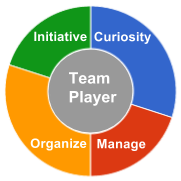
\includegraphics[scale=0.62]{img/personal.png}
    ~
    
%\end{tcolorbox}
\end{aside}
\section{Education}
\begin{entrylist}
    \entry
    {2016 - Now}
    { BSc(Eng) Electrical and Information Engineering}
    {University of the Witwatersrand}
    %{{\textbf{\textcolor{black}{\hlcyan{University of the Witwatersrand}}}}}
    {Main subjects: Software Development, Data Intensive Computing in Data Science, Data \& Information Management, Signal Processing, Network Systems, Microprocessors, Electronics.\\
    Current Year: $4^{th}$}
  \entry
    {2011 - 2015}
    {Matriculation}
    {Tlakale Mashashane Commercial High School }
    %{{\textbf{\textcolor{black}{\hlcyan{Tlakale Mashashane Commercial High School }}}}}
    {Highest Grade: Grade 12.\\
    Main subjects: Mathematics, Physical Sciences, Accounting, Life Sciences, Sepedi HL, English FAL}
\end{entrylist}

\section{Experience}
\begin{entrylist}
 \entry{07/19 - Now}
        {Software Development Tutor}
        {University of the Witwatersrand}
        {Tutoring 3rd year Software Development students in Object-Oriented Programming ( such as Inheritance, Polymorphism, Abstraction, and Encapsulation) and Version Control using GitHub and Git. }

  \entry{02/18 - Now}
        {All Res Tutor}
        {University of the Witwatersrand}
        {Tutoring \& mentoring first year Engineering students on how to navigate and survive in the university field. The courses tutored are all the first year Engineering courses. }
 \entry{06/19 - 06/19}
        {Intern}
        {Derivco}
        {A week of developing online gambling games using technologies such as Node, Express, Angular and MongoDB. I was part of a group of 4 where we developed an online gambling game using NodeJS for the backend and Angular 7 for the front end. We used Trello for project management and GitHub \& Git for version control.}
  \entry
    {11/18 - 12/18}% && 11/2018 - 12/2018\\}
    {Intern}
    {Wits Business Intelligence Services}
    {Development and application of Machine Learning models using techniques such as Clustering, Random Forest, Decision Trees and Naive Bayes to predict and classify data using KNIME, Anaconda \& Python.}
  \entry
    {06/18 - 07/18}% && 11/2018 - 12/2018\\}
    {Intern}
    {Wits Business Intelligence Services}
    {Cleansing of Big Data, creation of data marts using ODI and SQL and the creation of a dashboard using Power BI.}
\end{entrylist}



\section{Certifications}
\begin{entrylist}
  \entry
    {12/2018}
    {Data Science Fundamentals}
    {Wits Business Intelligence Services}
    {\emph{Business Intelligence Concepts: Data Warehousing, Data Wrangling, Machine Learning (ML), ML Models, Data Mining, Data Analytics, Data Presentation}}
\end{entrylist}
\newpage
\section{Achievements}

\begin{entrylist}
    \entry{2019}{Discovery Gradhack Winner}{Discovery}
    {\vspace{-0.2cm}}
    \entry{2017}{Top 15\%}{University of the Witwatersrand}{\vspace{-0.2cm}}
    \entry{2017}{Dean's List}{University of the Witwatersrand}{\vspace{-0.2cm}}
    \entry{2016}{SAIEE Past President Scholarship}{SAIEE}{\vspace{-0.2cm}}
    \entry{2016}{University Entrance Scholarship}{University of the Witwatersrand}{\vspace{-0.2cm}}
    \entry{2015}{Top Matriculant}{Tlakale Mashashane Commercial High School}{\vspace{-0.2cm}}
    \entry{2015}{Cricket Team Captain}{Tlakale Mashashane Commercial High School}{\vspace{-0.2cm}}
\end{entrylist}

\section{Extra Curricular Activities}

\begin{entrylist}
    \entry{02/19 - Now}{Student Assist}{Wits CCDU}
    {Making students aware of vacation work opportunities and graduates aware of graduate recruitment programmes. Assisting with the organisation of career open days, wellness campaigns and company open days.}
    \entry{}{Cricket Player}{}{\vspace{-0.2cm}}
    \entry{}{Member of Equal Education}{}{\vspace{-0.2cm}}
    \entry{}{Member of SAIEE}{}{\vspace{-0.2cm}}
\end{entrylist}


\section{References}
\begin{entrylist}
    \entry{}{Innocent Mamvura}{Data Scientist, Wits Business Intelligence Services}{
    Cell:  083 400 6855\\
    Email:  \href{mailto:innocentmamvura9@gmail.com}{innocentmamvura9@gmail.com}}
     \entry{}{Dr. Stephen Levitt}{Software Development Lecture, School of Electrical \& Information Engineering}{
    Tell: (011) 717 7209\\
    Email:  \href{mailto:Stephen.Levitt@wits.ac.za}{Stephen.Levitt@wits.ac.za}}
\end{entrylist}
%\emph{Wits Business Intelligence Services}
%




%\begin{flushleft}
%\emph{January 14th, 2014}
%\end{flushleft}
%\begin{flushright}
%\emph{Carmine Benedetto}
%\end{flushright}

%%% This piece of code has been commented by Karol Kozioł due to biblatex errors. 
% 
%\printbibsection{article}{article in peer-reviewed journal}
%\begin{refsection}
%  \nocite{*}
%  \printbibliography[sorting=chronological, type=inproceedings, title={international peer-reviewed conferences/proceedings}, notkeyword={france}, heading=subbibliography]
%\end{refsection}
%\begin{refsection}
%  \nocite{*}
%  \printbibliography[sorting=chronological, type=inproceedings, title={local peer-reviewed conferences/proceedings}, keyword={france}, heading=subbibliography]
%\end{refsection}
%\printbibsection{misc}{other publications}
%\printbibsection{report}{research reports}

\end{document}
